% !TEX root=report.tex
\section{Prediction Model}
\label{sec:model}

\begin{figure}[ht]
\centering
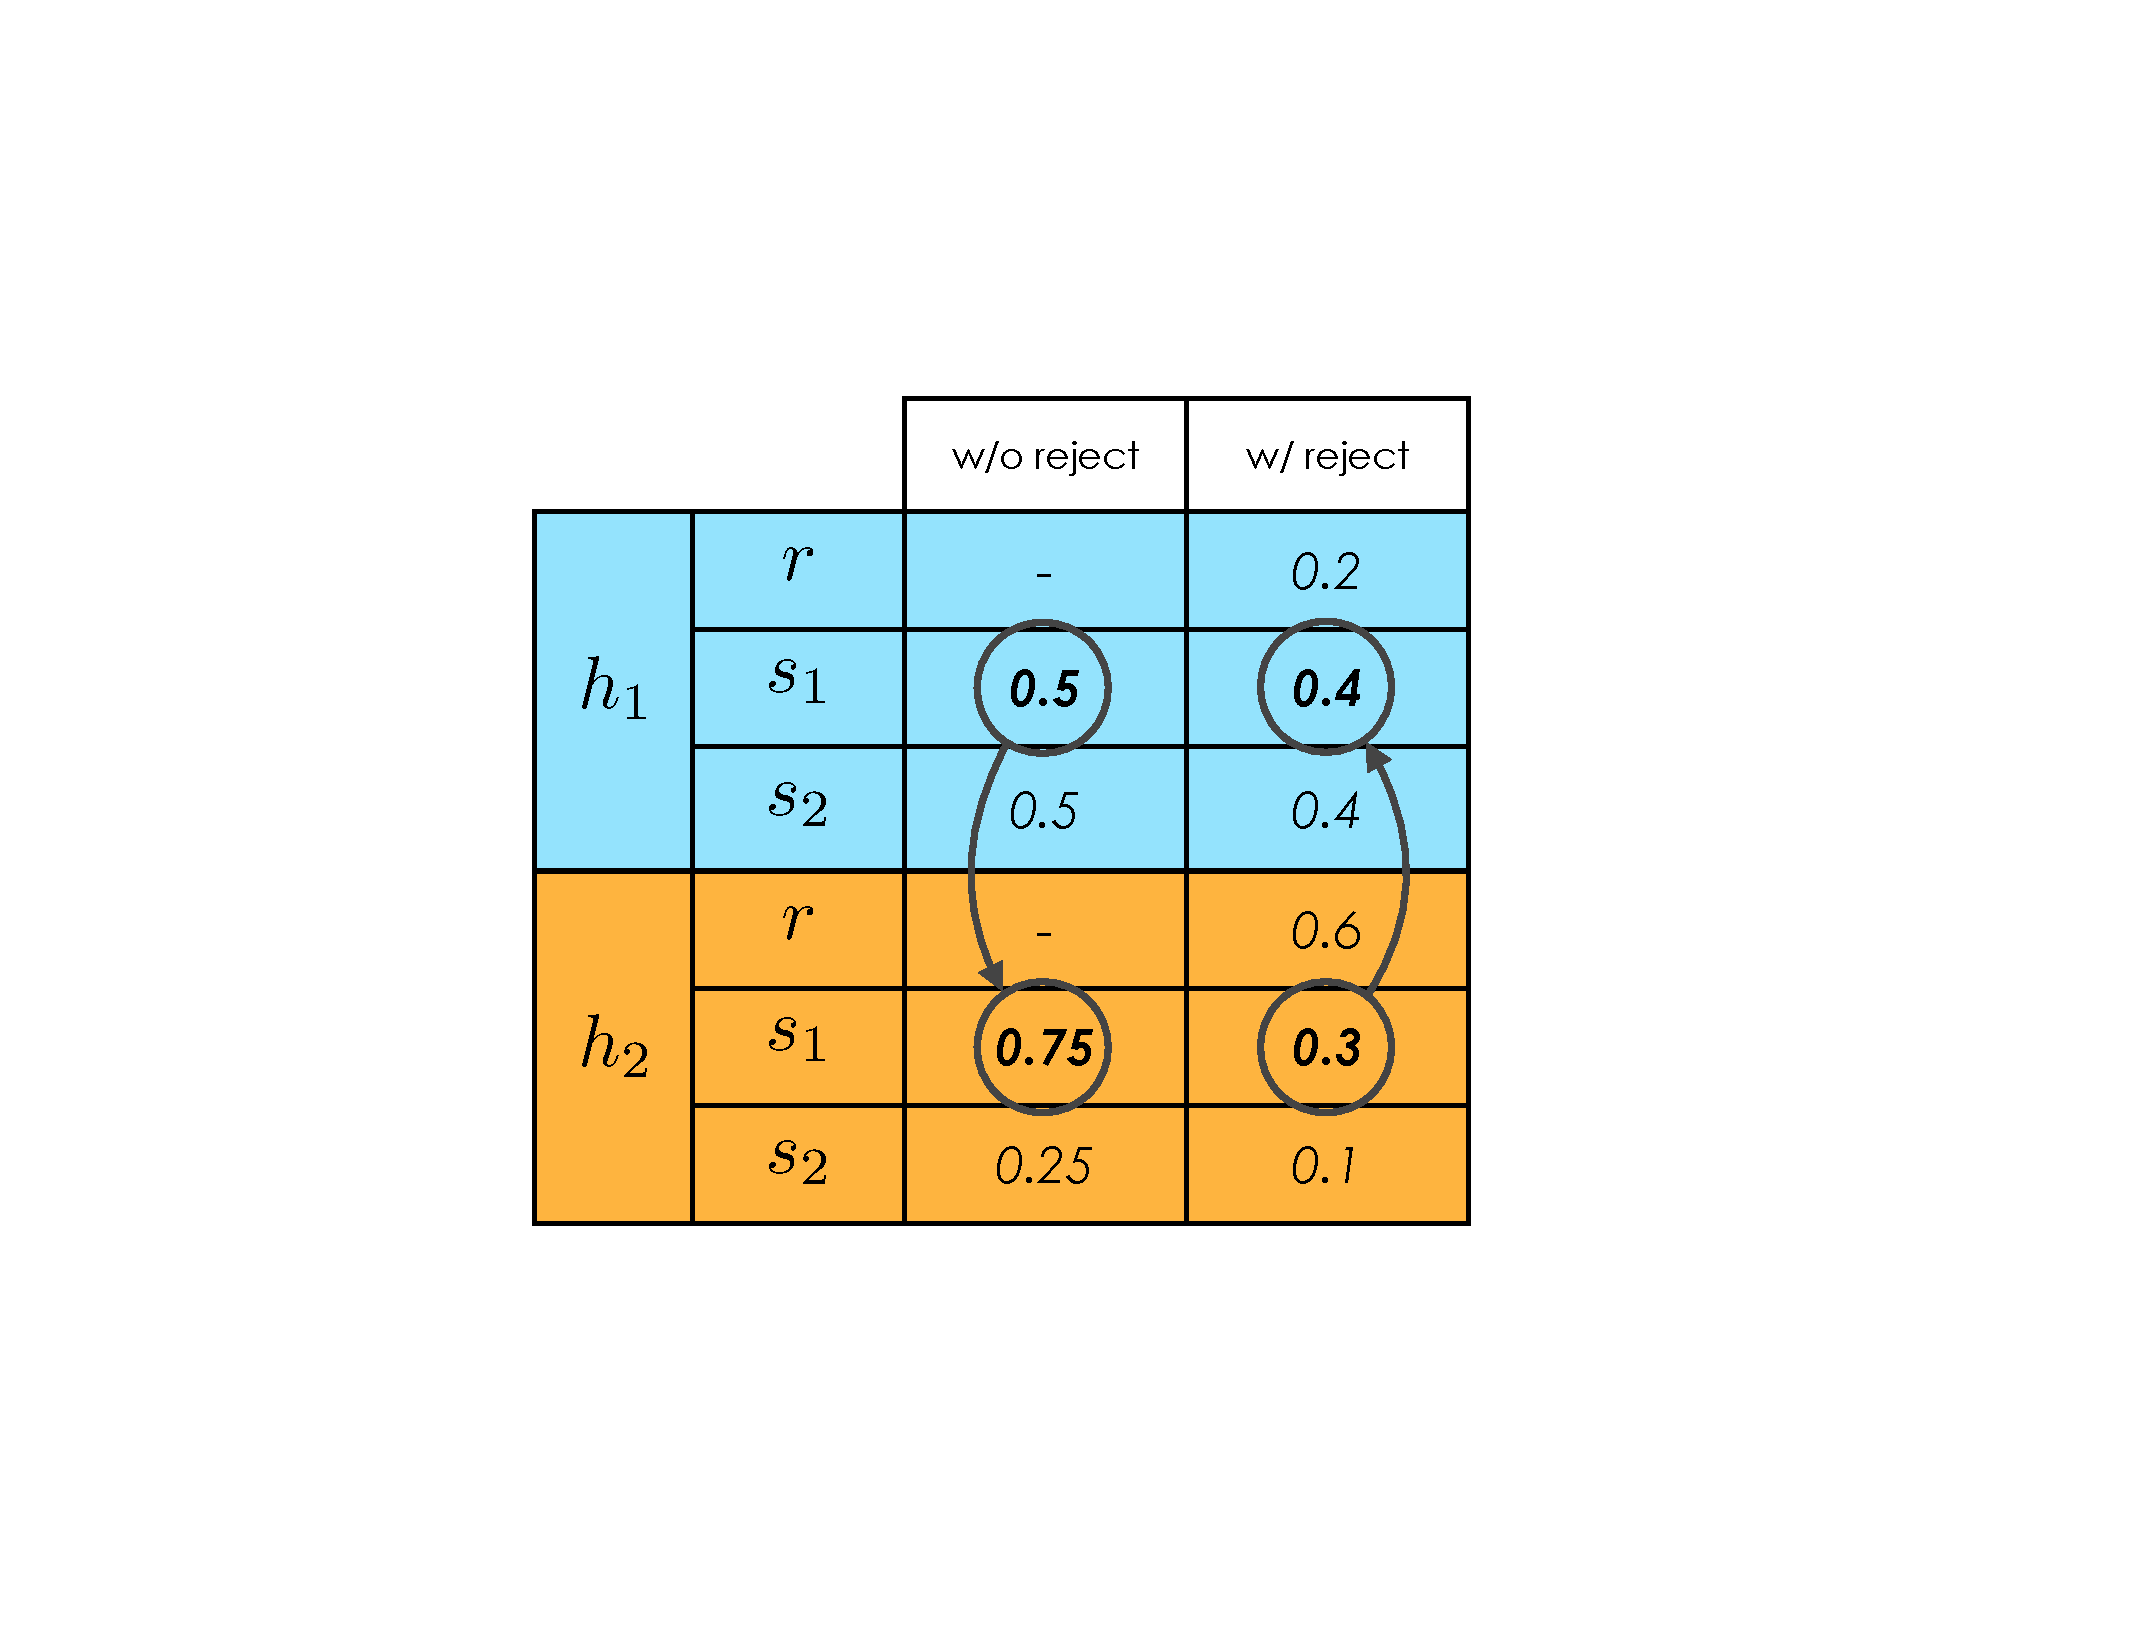
\includegraphics[width=0.6\linewidth]{figures/reject_vs_no_reject.pdf}
\caption{
Example of a case where modeling the reject option results in vastly different recommendation behavior.
Consider surfer $s_1$'s perspective: without modeling the reject option, $h_2$ looks more likely to accept $s_1$.
When modeling the reject option, however, the probabilities change and $h_1$ is now more likely to accept $s_1$, due to the ability to model how picky $h_2$ actually is.}
\label{fig:reject_vs_no_reject}
\end{figure}

We predict the probability that a host $h$ chooses the surfers $s_{k^*}$ among a competitorset $S=\{ s_1, \dots, s_n\}$ or that he rejects all of them using the following logistic model:
\begin{eqnarray}
p(s_k | h, S) &=& \frac{\exp(\theta^T \Phi(s_k,h))}{\sum_{s_j \in S} \exp(\theta^T \Phi(s_j,h)) + \exp(r)} \\
p(\text{reject} | h, S) &=& \frac{\exp(r)}{\sum_{s_j \in S} \exp(\theta^T \Phi(s_j,h)) + \exp(r)}
\end{eqnarray}
In this formulation, each surfer $s_k$ receives a score $\exp(\theta^T \Phi(s_k,h))$ modeling the natural competition between multiple surfers that requested to stay with the host. In the end, we predict that the surfer with the highest score wins, or that everybody gets rejected if the rejectscore $\exp{(r)}$ is largest. 
Further, we implicitly learn a bias term by appending a one to the feature representation $\Phi(s_k,h)$.
Note, however, that this is not exactly the standard multinomial logistic regression model since in our case we have the same parameters but we have different features for the different ``classes'' (i.e. surfers).

Even though we essentially just rank the candidates for the host that sent a couchrequest it is still important to model the possibility of rejection. It enables us to model actual probabilities that are very important from the perspective of the surfers. For them, we rank the different host in order of the likelihood that their couchrequest to these hosts would be successful. Because we compare different hosts to each other here their pickiness actually matters to the surfer. See Figure \ref{fig:reject_vs_no_reject} for an example where modeling 

The parameters (to be learned) for this model capture what hosts prefer in surfers and their request, i.e. their language, nationality, age, gender etc. Because the feature $\Phi(s_k,h)$ depends on both the surfer and the host we also model that i.e. Americans like to host surfers from certain countries and that hosts generally prefer to have a language in common with the couchsurfer.

These preferences might be very different from host to host though. Also, some hosts might be more picky than others rejecting almost all requests and we should be able to capure that, too. Therefore, we introduce host-specific parameters $\theta_h$ and $r_h$ to model these effects. Because we have millions of hosts storing all these parameters explicitly would require tens of gigabytes of memory. % TODO should the hashing trick get it's own section? I would say explain it a bit in related work and a bit here again
Since this is infeasible we make use of the hashing trick to hash the parameters into an array of predefined size (allowing for collisions between parameters). Thereby, we can control how much memory we want to allocate for personalization. This trick has been successfully applied e.g. for spam classification \cite{Attenberg2009}.
Including personalized parameters leads to the following updated model:
\begin{eqnarray}
p(s_k | h, S) &=& \frac{\exp((\theta + \theta_h)^T \Phi(s_k,h))}{\sum_{s_j \in S} \exp((\theta + \theta_h)^T \Phi(s_j,h)) + \exp(r + r_{h})} \\
p(\text{reject} | h, S) &=& \frac{\exp(r+r_{h})}{\sum_{s_j \in S} \exp((\theta + \theta_h)^T \Phi(s_j,h)) + \exp(r + r_{h})}
\end{eqnarray}
As an error measure we use the negative log-likelihood of the data with $l_2$-penalty on the parameters for regularization. In our Stochastic Gradient Descent (SGD), we randomly sample a host $h$ and a competitorset $S=\{ s_1, \dots, s_n\}$. There are two cases: either there is one surfer $s_{k^*}$ that got accepted, or everybody got rejected. We obtain the following update equations for SGD where $\lambda_1, \lambda_2$ are regularization parameters and $\eta$ is the learning rate

1. Case: Some surfer $s_{k^*}$ gets chosen (no reject):
\begin{eqnarray}
\theta &\leftarrow& (1- \eta \lambda_1) \theta - \eta (\sum_{j \in S_n} p(s_j | h, S) \Phi(s_j,h_n) - \Phi(s_{k^*},h_n))\\
r &\leftarrow& (1- \eta \lambda_2) r - \eta p(\text{reject} | h_n, S_n)
\end{eqnarray}

2. Case: No surfer gets chosen (reject):
\begin{eqnarray}
\theta &\leftarrow& (1- \eta \lambda_1) \theta - \eta (\sum_{j \in S_n} p(s_k | h, S) \Phi(s_j,h_n))\\
r &\leftarrow& (1- \eta \lambda_2) r - \eta (p(\text{reject} | h_n, S_n)-1)
\end{eqnarray}

The update equations for $\theta_h$ and $r_h$ are the same as the ones for $\theta$ and $r$, respectively, but they are only updated for the current host $h$. 
Also note that these update equations intuitively make sense . For $\theta$ we essentially increase the contribution from the features of the winner and decrease it for all the losers always according to their probability of being chosen. This means that if the model did a bad prediction we update our parameters more than normally. For $r$ it is similar in the sense that we increase it whenever everybody actually got rejected and decrease it if we had a winner.


%%%%%%%%%%%%%%%%%%%%%%%%%%%
% this is where the old stuff starts
%-----------------OLD STUFF------
%
%\begin{eqnarray}
%p(s_k | h_n, S_n) &=& \frac{\exp(\theta^T \Phi(s_k,h_n))}{\sum_{j \in S_n} \exp(\theta^T \Phi(s_j,h_n)) + \exp(r + r_{h_n})} \\
%p(\text{reject} | h_n, S_n) &=& \frac{\exp(r+r_{h_n})}{\sum_{j \in S_n} \exp(\theta^T \Phi(s_j,h_n)) + \exp(r + r_{h_n})}
%\end{eqnarray}
%Note that $\Phi(s_k,h_n)$ also implicitly depends on the couchrequest (e.g. date, whether the host is already booked, etc.).
%
%To have hostspecific parameters we would replace $\theta$ by $\theta + \theta_h$. 
%
%Further, we want to add regularization for $\theta, \theta_h, r_{h_n}$.
%
%Error (negative log likelihood)
%\begin{eqnarray}
%E(\theta, r, r_{h_n}) &=& - \log p(\{s_k\} | \{h_n\}, \{S_n\})\\
%&=& - \log [ \prod_{n=1}^N \prod_{k=1}^K p(s_k | h_n, S_n)^{t_{nk}}]\\
%&=&  - \sum_{n=1}^N \sum_{k=1}^K t_{nk} \log p(s_k | h_n, S_n)
%\end{eqnarray}
%
%To derive the gradient descent update steps we will take derivatives of $E(\theta, r, r_{h_n})$ wrt. $\theta, r, r_{h_n}$. Because we will do stochastic gradient descent we will basically ignore the sum over $n$ in the end (over different ``competitor sets $S_n$'') and just choose one at random. Note that here, we can just sample uniformly from all sets or sample a host first, and given that host, sample on of his sets. The latter will achieve that all hosts have the sample influence on the learning but we will have to discuss/test whether we actually want that.
%
%We generally have:
%\begin{eqnarray}
%\frac{d}{d \theta} E(\theta, r, r_{h_n}) &=& - \sum_{n=1}^N \sum_{k=1}^K t_{nk} \frac{d}{d \theta}  \log p(s_k | h_n, S_n) \\
%&=& - \sum_{n=1}^N \sum_{k=1}^K t_{nk} \frac{1}{p(s_k | h_n, S_n)} \frac{d}{d \theta} p(s_k | h_n, S_n)
%\end{eqnarray}
%
%Now we look at the individual derivatives of $p(s_k | h_n, S_n)$ and $p(\text{reject} | h_n, S_n)$.
%
%1. Case: Some surfer $s_k$ gets chosen (no reject):
%\begin{eqnarray}
%\frac{d}{d \theta} p(s_k | h_n, S_n) = \frac{d}{d \theta} \frac{\exp(\theta^T \Phi(s_k,h_n))}{\sum_{j \in S_n} \exp(\theta^T \Phi(s_j,h_n)) + \exp(r + r_{h_n})} \\
%= \frac{\Phi(s_k,h_n) [\sum_{j \in S_n} \exp(\theta^T \Phi(s_j,h_n)) + \exp(r + r_{h_n})]}{\sum_{j \in S_n} \exp(\theta^T \Phi(s_j,h_n)) + \exp(r + r_{h_n})} \\
%- \frac{\exp(\theta^T \Phi(s_k,h_n)) [\sum_{j \in S_n} \Phi(s_j,h_n) \exp(\theta^T \Phi(s_j,h_n))]}{\sum_{j \in S_n} \exp(\theta^T \Phi(s_j,h_n)) + \exp(r + r_{h_n})}\\
%= \Phi(s_k,h_n) p(s_k | h_n, S_n) - p(s_k | h_n, S_n) \frac{\sum_{j \in S_n} \Phi(s_j,h_n) \exp(\theta^T \Phi(s_j,h_n))}{\sum_{j \in S_n} \exp(\theta^T \Phi(s_j,h_n)) + \exp(r + r_{h_n})}\\
%= p(s_k | h_n, S_n) (\Phi(s_k,h_n) - \sum_{j \in S_n} w_{jn} \Phi(s_j,h_n))
%\end{eqnarray}
%where $w_{jn}=\frac{\exp(\theta^T \Phi(s_j,h_n))}{\sum_{j \in S_n} \exp(\theta^T \Phi(s_j,h_n)) + \exp(r + r_{h_n})}$.
%
%Thus, we get:
%\begin{eqnarray}
%\frac{d}{d \theta} E(\theta, r, r_{h_n}) = - \sum_{n=1}^N \sum_{k=1}^K t_{nk} \frac{1}{p(s_k | h_n, S_n)} \frac{d}{d \theta} p(s_k | h_n, S_n)\\
%= - \sum_{n=1}^N \sum_{k=1}^K t_{nk} (\Phi(s_k,h_n) - \sum_{j \in S_n} w_{jn} \Phi(s_j,h_n)) \\
%= \sum_{n=1}^N (\sum_{j \in S_n} w_{jn} \Phi(s_j,h_n) - \Phi(s_{k^*},h_n))
%\end{eqnarray}
%where $s_{k^*}$ is the surfer that got accepted from the competitor set $S_n$.
%
%Similarly, taking the derivative wrt. $r$ ($r_{h_n}$ should be exactly the same) we obtain:
%\begin{eqnarray}
%\frac{d}{d r} p(s_k | h_n, S_n) = -  p(s_k | h_n, S_n)  \frac{\exp(r + r_{h_n})}{\sum_{j \in S_n} \exp(\theta^T \Phi(s_j,h_n)) + \exp(r + r_{h_n})}
%\end{eqnarray}
%Thus, we get:
%\begin{eqnarray}
%\frac{d}{d r} E(\theta, r, r_{h_n}) = - \sum_{n=1}^N \sum_{k=1}^K t_{nk} \frac{1}{p(s_k | h_n, S_n)} \frac{d}{d r} p(s_k | h_n, S_n)\\
%= \sum_{n=1}^N \sum_{k=1}^K t_{nk} \frac{\exp(r + r_{h_n})}{\sum_{j \in S_n} \exp(\theta^T \Phi(s_j,h_n)) + \exp(r + r_{h_n})} \\
%= \sum_{n=1}^N \frac{\exp(r + r_{h_n})}{\sum_{j \in S_n} \exp(\theta^T \Phi(s_j,h_n)) + \exp(r + r_{h_n})}
%\end{eqnarray}
%
%
%
%2. Case: No surfer gets chosen (reject):
%\begin{eqnarray}
%\frac{d}{d \theta} p(\text{reject} | h_n, S_n) = \frac{d}{d \theta} \frac{\exp(r+r_{h_n})}{\sum_{j \in S_n} \exp(\theta^T \Phi(s_j,h_n)) + \exp(r + r_{h_n})}\\
%= - p(\text{reject} | h_n, S_n) \frac{\sum_{j \in S_n} \Phi(s_j,h_n) \exp(\theta^T \Phi(s_j,h_n))}{\sum_{j \in S_n} \exp(\theta^T \Phi(s_j,h_n)) + \exp(r + r_{h_n})} \\
%= - p(\text{reject} | h_n, S_n) \sum_{j \in S_n} w_{jn} \Phi(s_j,h_n)
%\end{eqnarray}
%Thus, we get:
%\begin{eqnarray}
%\frac{d}{d \theta} E(\theta, r, r_{h_n}) = - \sum_{n=1}^N \sum_{k=1}^K t_{nk} \frac{1}{p(\text{reject} | h_n, S_n)} \frac{d}{d \theta} p(\text{reject} | h_n, S_n)\\
%= \sum_{n=1}^N (\sum_{j \in S_n} w_{jn} \Phi(s_j,h_n))
%\end{eqnarray}
%
%
%
%Again, taking the derivative wrt. $r$ ($r_{h_n}$ should be exactly the same) we obtain:
%\begin{eqnarray}
%\frac{d}{d r} p(\text{reject} | h_n, S_n) = p(\text{reject} | h_n, S_n) - p(\text{reject} | h_n, S_n)^2\\
%= p(\text{reject} | h_n, S_n) (1 - p(\text{reject} | h_n, S_n))\\
%\end{eqnarray}
%Thus, we get:
%\begin{eqnarray}
%\frac{d}{d r} E(\theta, r, r_{h_n}) = - \sum_{n=1}^N \sum_{k=1}^K t_{nk} \frac{1}{p(\text{reject} | h_n, S_n)} \frac{d}{d \theta} p(\text{reject} | h_n, S_n)\\
%= \sum_{n=1}^N (p(\text{reject} | h_n, S_n)-1)
%\end{eqnarray}
%
%
%\paragraph{The final update equations}
%
%Finally, for stochastic gradient descent the following update equations hold. We simply sample a host $h_n$ and competitor set $S_n$. Note that the following equations do not contain regularization, yet (although trivial).
%
%1. Case: Some surfer $s_{k^*}$ gets chosen (no reject):
%\begin{eqnarray}
%\theta \leftarrow \theta - \eta (\sum_{j \in S_n} w_{jn} \Phi(s_j,h_n) - \Phi(s_{k^*},h_n))\\
%r \leftarrow r - \eta \frac{\exp(r + r_{h_n})}{\sum_{j \in S_n} \exp(\theta^T \Phi(s_j,h_n)) + \exp(r + r_{h_n})}
%\end{eqnarray}
%where, again, $w_{jn}=\frac{\exp(\theta^T \Phi(s_j,h_n))}{\sum_{j \in S_n} \exp(\theta^T \Phi(s_j,h_n)) + \exp(r + r_{h_n})}$.
%
%2. Case: No surfer gets chosen (reject):
%\begin{eqnarray}
%\theta \leftarrow \theta - \eta (\sum_{j \in S_n} w_{jn} \Phi(s_j,h_n))\\
%r \leftarrow r - \eta (p(\text{reject} | h_n, S_n)-1)
%\end{eqnarray}
%
%For $l_2$-regularization, e.g. of $\theta$, just add $- \eta \lambda \theta$ to the update equation.
%
